\documentclass[12pt,a4paper]{article}
\usepackage[UTF8]{ctex}
\usepackage{amsmath,amssymb}
\usepackage{listings}
\usepackage{xcolor}
\usepackage{hyperref}
\usepackage{geometry}
\usepackage{graphicx}
\geometry{margin=2.5cm}

\lstdefinestyle{python}{
  language=Python,
  basicstyle=\ttfamily\small,
  keywordstyle=\color{blue}\bfseries,
  commentstyle=\color{gray},
  stringstyle=\color{red},
  showstringspaces=false,
  breaklines=true,
  frame=single,
  backgroundcolor=\color{gray!10}
}

\title{QAOA / 量子近似优化算法}
\author{QuoNic}
\date{}

\begin{document}
\maketitle

\begin{center}
\textbf{Algorithms / 算法} | 难度：高级 | 预计时间：20 分钟
\end{center}

\tableofcontents
\newpage

\section{为什么需要？}

QAOA 是解决组合优化问题的量子算法，是近期量子设备上最有前景的应用之一。

\subsection{经典局限}
\b\begin{itemize}
  \item NP-hard 问题（如 MaxCut）经典算法只能近似求解
  \item 经典近似算法有性能保证的上限
  \item 对于大规模问题，经典方法效率低
\end{itemize}

\subsection{量子优势}
\b\begin{itemize}
  \item QAOA 可以提供比经典近似算法更好的解
  \item 对噪声有鲁棒性，适合近期量子设备
  \item 理论上可以达到最优解
\end{itemize}

\subsection{实际应用}
\b\begin{itemize}
  \item MaxCut 问题
  \item 图着色问题
  \item 旅行商问题
  \item 供应链优化
\end{itemize}

\section{快速上手}

\begin{lstlisting}[style=python]
from quonic.algorithms import qaoa

# Define MaxCut problem
graph = [(0,1), (1,2), (2,3), (3,0)]

# Run QAOA
result = qaoa(graph, p=2, optimizer="cobyla")
print(f"MaxCut value: {result.maxcut_value}")
print(f"Solution: {result.solution}")
\end{lstlisting}

\textbf{预期输出}：
\begin{verbatim}
MaxCut value: 4
Solution: [1, 0, 1, 0]
\end{verbatim}

\section{原理详解}

\subsection{电路图}

\begin{center}
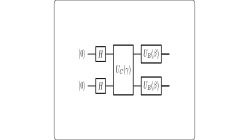
\includegraphics[width=0.6\textwidth]{../../images/qaoa_circuit.svg}
\end{center}

\subsection{数学推导}

QAOA 优化问题的目标函数：
\begin{equation}
C(z) = \sum_{(i,j) \in E} w_{ij} (1 - z_i z_j)
\end{equation}

QAOA 电路：
\begin{equation}
|\gamma, \beta\rangle = \prod_{l=1}^{p} e^{-i\beta_l B} e^{-i\gamma_l C} |+\rangle^{\otimes n}
\end{equation}

其中 $B = \sum_i X_i$ 是混合算子，$C$ 是问题算子。

\subsection{几何解释}

QAOA 在参数空间中寻找最优的 $(\gamma, \beta)$，使得测量结果的期望值最大化。

\section{代码详解}

\begin{lstlisting}[style=python]
from quonic.algorithms import qaoa

# qaoa(graph, p, optimizer)
# graph: list of edges (i, j)
# p: number of QAOA layers
# optimizer: classical optimizer
result = qaoa(graph, p=2, optimizer="cobyla")

# result.maxcut_value: optimal cut value
# result.solution: bit string solution
# result.params: optimized parameters
print(f"MaxCut: {result.maxcut_value}")
\end{lstlisting}

\section{进阶用法}

\subsection{场景 1：不同层数}

\begin{lstlisting}[style=python]
# More layers for better approximation
result_p1 = qaoa(graph, p=1)
result_p2 = qaoa(graph, p=2)
result_p4 = qaoa(graph, p=4)
\end{lstlisting}

\subsection{场景 2：加权图}

\begin{lstlisting}[style=python]
# Weighted graph
graph = [(0,1,2.0), (1,2,1.5), (2,3,3.0)]
result = qaoa(graph, p=2)
\end{lstlisting}

\subsection{场景 3：其他优化问题}

\begin{lstlisting}[style=python]
# Traveling salesman problem
from quonic.optimization import tsp
result = tsp(cities, optimizer="qaoa")
\end{lstlisting}

\section{适用场景}

\subsection{MaxCut 问题}

QAOA 最初就是为 MaxCut 问题设计的。

\subsection{组合优化}

QAOA 可以用于各种组合优化问题。

\subsection{机器学习}

QAOA 可以用于量子机器学习中的特征选择。

\section{常见问题}

\subsection{QAOA 和 VQE 有什么区别？}

QAOA 用于组合优化（离散变量），VQE 用于量子化学（连续变量）。

\subsection{QAOA 需要多少层？}

层数 $p$ 越大，近似比越好。但更多的层意味着更多的参数需要优化。

\subsection{QAOA 能保证最优解吗？}

理论上，当 $p \to \infty$ 时，QAOA 可以达到最优解。但实际中 $p$ 有限，只能近似求解。

\section{学习路径}

\subsection{前置知识}
\b\begin{itemize}
  \item 组合优化基础
  \item 量子电路
  \item 变分方法
\end{itemize}

\subsection{继续学习}
\b\begin{itemize}
  \item VQE（量子化学）
  \item 量子退火
  \item 量子机器学习
\end{itemize}

\section{完整示例代码}

\subsection{示例 1：基本 QAOA}

\begin{lstlisting}[style=python]
from quonic.algorithms import qaoa

graph = [(0,1), (1,2), (2,3), (3,0)]
result = qaoa(graph, p=2, optimizer="cobyla")
print(f"MaxCut: {result.maxcut_value}")
\end{lstlisting}


\section{下载}

\begin{itemize}
  \item [qaoa.py](https://github.com/ChrisLee0721/QuoNic/blob/main/examples/qaoa/qaoa.py)
\end{itemize}

\end{document}
